\documentclass[11pt, twocolumn, a4paper]{article}

\usepackage{graphicx}

\setlength{\oddsidemargin}{0.0 cm}
\setlength{\evensidemargin}{0.0 cm}
\setlength{\topmargin}{-1cm}
\setlength{\textheight}{24 cm}
\setlength{\textwidth}{16 cm}

\newcommand{\ttbarm}{\mathrm{t \overline{t} \; }}
\newcommand{\ttbar}{$\mathrm{t \overline{t} \; }$}

\pagestyle{plain}

\setlength{\parindent}{0in}

\usepackage[
  locale=DE,
  separate-uncertainty=true,
  decimalsymbol=.,
  per-mode=symbol-or-fraction,
]{siunitx}
\usepackage{amsmath,amssymb}

\begin{document}

\author{Salvatore La Cagnina}

\title{Summary of `CMS Collaboration, {\it Measurements of the $\mathrm{t\overline{t}}$ production cross section using events in the $\mathrm{e\mu}$ final state in pp collisions at $\sqrt{s} = \SI{13}{TeV}$}'}

\maketitle
\begin{small}
{\bf Abstract}
The paper describes the analysis of \ttbar events with $\mathrm{e\mu}$ final state in order to measure the \ttbar production cross section \cite{paper}.
It uses data provided by the CMS experiment from pp collisions at a center of mass energy of $\SI{13}{TeV}$ with an integrated luminosity of $\SI{2.2}{fb^{-1}}$.
The selection of this analysis consists of having an opposite signed (OS) pair of electron and muon together with two or more jets of which at least one resulted from the hadronization of a $b$ quark.
The measured cross section for the \ttbar production is \! $\sigma _{\ttbarm}={\SI[parse-numbers=false]{815 \pm 9 (stat) \pm 38 (syst) \pm 19 (lumi)}{\pico\barn}}$ \! which is in agreement with the standard model prediction.
\end{small}\\

Measuring the \ttbar production at the CMS experiment at the LHC yields multiple beneficial information.
It tests the prediction provided by the QCD and can add constrains on the parton distribution functions. 
%##########################################################################
%Additionally, it grants information about the top quark pole mass but the most important reason precise data about the \ttbar production is necessary is the search for BSM physics since \ttbar is the dominant background in those analysis. %TODO##################################################
Additionally, it grants information about the top quark pole mass.
However, the most important reason to determine the \ttbar production cross section is its contribution as background in search for BSM physics.
%#######################################################################
For this analysis the full data set of 2015 from the CMS experiment is used providing a data set corresponding to an inverse luminosity of $\SI{2.2}{fb^{-1}}$ recorded with a center of mass energy of $\sqrt{s} = \SI{13}{TeV}$.
This corresponds to an increase of a factor $50$ in statistics compared to the original analysis \cite{Khachatryan:2015uqb}.

The CMS experiment is an experiment at the LHC at CERN used to analyze pp collisions.
The silicon pixel detector of the CMS detector covers $0 < \Phi < 2 \pi$ azimuth and a pseudorapidity of $| \eta | < 2.5$.
In order to detect jets and electrons, the lead tungstate crystal electromagnetic and the brass and scintillator hadron calorimeter are used.
Muons can be detected using the gas-ionization detectors outside the solenoid.%################################################
Signal and background events are simulated with different Monte Carlo (MC) event generators such as \texttt{POWHEG},\texttt{PYTHIA},\texttt{HERWIG++} and \texttt{MG5\_aMC}.
The Standard Model prediction is determined with \texttt{TOP++} for a top quark mass of $m_t = \SI{172.5}{GeV}$ and is calculated to be $\sigma _\ttbarm = \SI[parse-numbers=false]{832^{+20}_{-29} (scales) \pm 35 (PDF + \alpha_s)}{\pico\barn}$.

In order to suppress most background and to access the desired decay channel a certain selection is chosen.
The selection consists of the requirement of one isolated electron, one isolated muon with opposite electric charge, a transverse momentum $p_T > \SI{20}{GeV}$ and $| \eta | < 2.4$.
The isolation criteria is based on the sum of the momentum of the reconstructed particles in a cone around the lepton subtracting its contribution.
Furthermore, two or more jets with ${p_T > \SI{30}{GeV}}$ and ${| \eta | < 2.4}$ are necessary for a \ttbar candidate and an invariant mass of the electron and the muon of ${m_{e\mu} > \SI{20}{GeV}}$.
Finally, due to the nature of the decay of \ttbar into a bottom quark + antiquark at least one jet is required to be identified as a result of the hadronization of a $b$ quark.
This constrain reduces the amount of background events created by Drell-Yan (DY) and W+Jets events.

The main background processes for the $e \, \mu$ decay channel of \ttbar are single top quark production, Drell-Yan (DY) processes and events containing two or more prompt leptons from vector boson decays, referred to as VV events.
In order to calculate the result for the cross section a proper estimate for the number of background events is essential.
Therefore, multiple methods like the $"R_\mathrm{out/in}"$ method for the DY events or a same-sign to opposite-sign comparison for nonprompt leptonic background is used.

In order to make a appropriate estimation for the cross section systematic uncertainties have to be considered.
Some of the major contributions are caused by uncertainties due to the jet energy scale, the lepton efficiencies, the \ttbar NLO generator from the modeling and the uncertainty caused by the luminosity.
The total systematic uncertainty adds up to $\SI{43.0}{\pico\barn}$ which corresponds to a relative uncertainty of $\SI{5.3}{\%}$.

The cross section is calculated with a event counting method using the formula
\begin{equation*}
	\sigma _{\ttbarm} = \frac{N - N_{\mathrm{B}}}{\mathcal{A} \mathcal{L}}.
\end{equation*}
$N$ is the total number of events found in data after the selection is applied, $N_{\mathrm{b}}$ is the estimated number of background events extracted from modeling, $\mathcal{A}$ is the acceptance including the mean acceptance, the selection efficiency and the branching ratio of \ttbar into the $e^{\pm} \mu^{\mp}$ decay channel.
The value of $\mathcal{A}$ is $\SI{0.55(3)}{\%}$ and is determined from simulation with a top quark mass of $m_t = \SI{172.5}{GeV}$.
Finally, the resulting measured cross section is
\begin{align*}
	\sigma _\ttbarm = \SI[parse-numbers=false]{815 \pm 9 (stat) \pm 38 (syst) \pm 19 (lumi)}{\pico\barn}
\end{align*}
which is in agreement with measurements of the ATLAS Collaboration \cite{ATLAS} and the Standard Model prediction within one standard deviation.

\begin{thebibliography}{99}
\bibitem{paper} CMS Collaboration, Measurement of the $\mathrm{t\overline{t}}$ production cross section using events in the e$\mathrm{\mu}$ final state in pp collisions at ${\sqrt{s} = \SI{13}{TeV}}$, Eur. Phys. J. C 77 (2017) 172.
\bibitem{Khachatryan:2015uqb}
  CMS Collaboration,``Measurement of the top quark pair production cross section in proton-proton collisions at $\sqrt{s} =$ \SI{13}{TeV},''
  Phys.\ Rev.\ Lett.\  {\bf 116} (2016) No. 5
\bibitem{ATLAS}
  ATLAS Collaboration,
  ``Measurement of the $t\bar{t}$ production cross-section using $e\mu$ events with b-tagged jets in pp collisions at $\sqrt{s}$=13 TeV with the ATLAS detector,''
  Phys.\ Lett.\ B {\bf 761} (2016) 136
\end{thebibliography}



\end{document}


%\begin{figure}[ht!]
%  \begin{center}
%    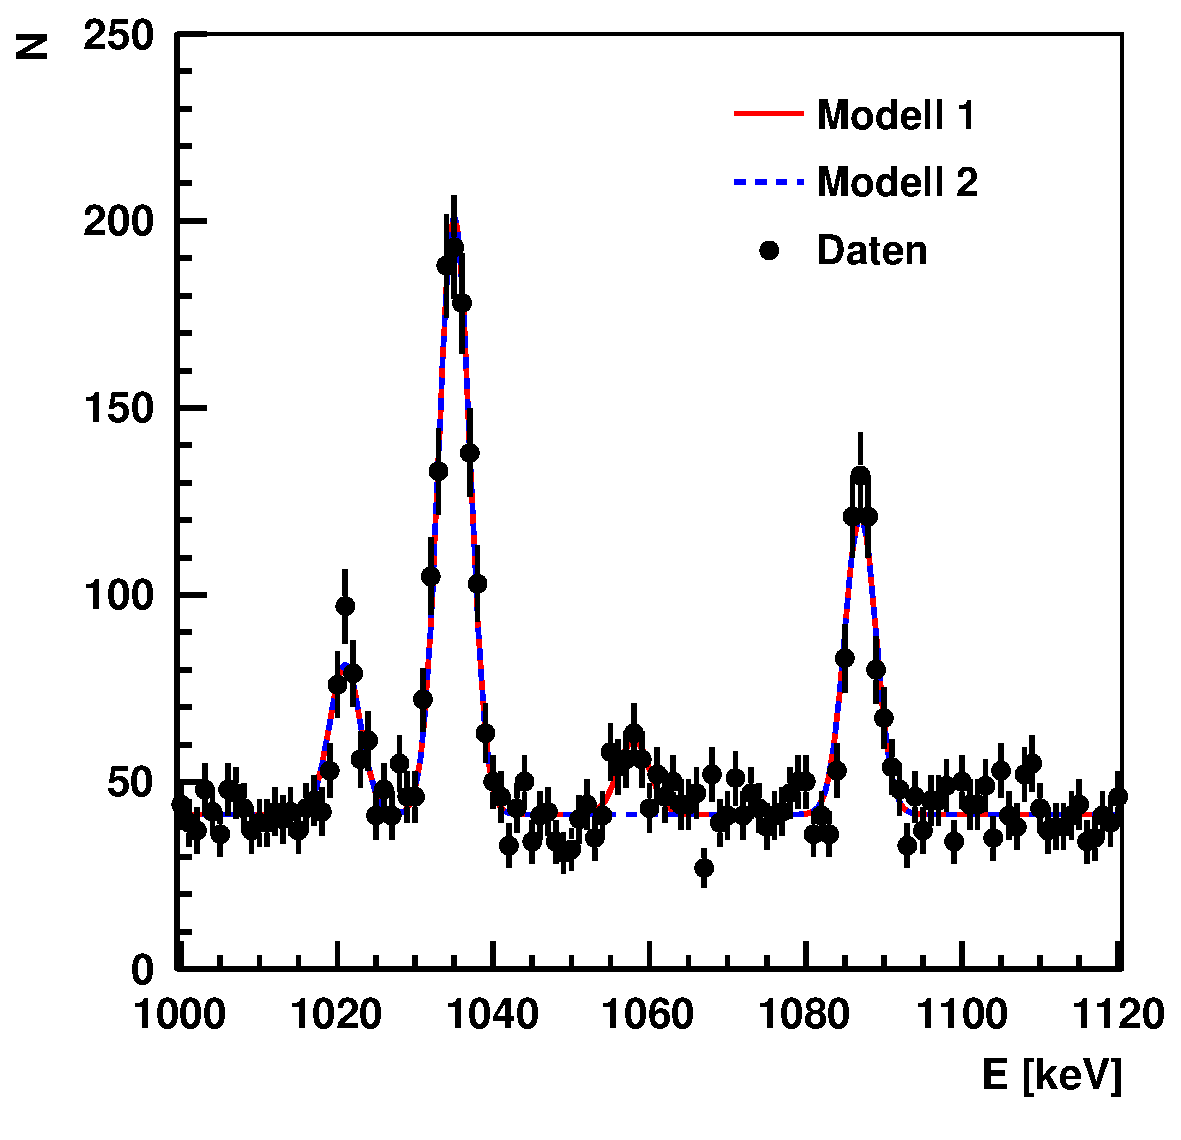
\includegraphics[width=0.5\textwidth]{plot.pdf}
%    \caption{A figure caption~\cite{brandt}.}
%    \label{fig:fig1}
%  \end{center}
%\end{figure}
